\documentclass[12pt, a4paper]{article}

\usepackage[margin=1in]{geometry}
\usepackage{graphicx}
\usepackage{hyperref}
\usepackage{booktabs}
\usepackage{enumitem}
\usepackage{subcaption}
\usepackage{xcolor}
\usepackage{titlesec}
\usepackage{parskip}
\usepackage{amsmath}
\usepackage{multirow}
\usepackage{float} 
\usepackage{longtable}

\titleformat{\section}{\large\bfseries}{\thesection.}{0.5em}{}
\titleformat{\subsection}{\normalsize\bfseries}{\thesubsection}{0.5em}{}
\titleformat{\subsubsection}{\normalsize\itshape}{\thesubsubsection}{0.5em}{}

\title{\textbf{Synthetic Specialization: Fine-Tuning and Compressing Foundation Models for Domain-Specific Tasks} \\ \large A Case Study in Warehouse Safety Hazard Detection}
\author{Jaskirat Singh Sohal \\ CIS*4900, University of Guelph \\ Supervisor: Prof.\ John Akinyemi}
\date{April 2026}

\begin{document}
\maketitle

% ============================================================
\begin{abstract}
% ============================================================

Large foundation models, whether for vision, language, or both, achieve impressive zero-shot performance on general tasks but often fall short on specialized domains where expert knowledge is required. We propose \textit{synthetic specialization}: a pipeline where AI-generated synthetic data is used to fine-tune and compress a foundation model into a small, fast, domain-specific expert. The approach requires no real-world training data collection, no manual annotation, and runs entirely on consumer hardware and free GPU services.

We demonstrate this pipeline on warehouse safety hazard detection, a domain where real hazard images are scarce and dangerous to stage. Starting from a 3D warehouse scene in Blender, we generate photorealistic drone-perspective images using Google Gemini, then inject realistic safety hazards (spills, forklift violations, improper stacking, aisle obstructions) through AI image editing. Dataset organization and metadata annotation were performed using Claude. This produces 913 fully labeled images across five categories.

We benchmark nine open-source Vision Language Models (VLMs) zero-shot across five prompt strategies and two inference modes (54 total runs), establishing that even the best zero-shot model (Qwen3.5-4B at 83.3\%) systematically fails on contextual hazards like pedestrian proximity to forklifts. We then fine-tune a 2.3-billion parameter Qwen3.5-2B model using LoRA on 2,521 multi-style training conversations. After Q4\_K\_M quantization, the resulting 1.8~GB model achieves 92.5\% accuracy with think mode at 4.2 seconds per image, outperforming zero-shot models up to 5 times its size. The full-precision variant reaches 94.1\%. Every accuracy figure was manually verified by reading all 186 test responses.

The contribution is not the model itself, but the pipeline. The same approach, generating synthetic training data with AI, fine-tuning a small model, quantizing for deployment, applies to any domain where real data is scarce but the target environment is known: medical imaging, document understanding, industrial inspection, agricultural monitoring, or any other specialized task. We show that \textit{small fine-tuned models consistently beat large generic models} when training data matches the deployment context, suggesting a paradigm shift from scaling model size to scaling data specificity.
\end{abstract}

% ============================================================
\section{Introduction}
% ============================================================

Foundation models have transformed artificial intelligence. Models like GPT-4, Claude, Gemini, and open-source alternatives such as Qwen, LLaMA, and Gemma demonstrate remarkable capabilities across a wide range of tasks without task-specific training. For vision-language tasks specifically, Vision Language Models (VLMs) can analyze images, answer questions about them, and produce detailed natural language descriptions, all from a single prompt.

However, a gap persists between general-purpose competence and domain-specific expertise. A VLM can describe what it sees in a warehouse image, but determining whether a worker standing near an active forklift constitutes an OSHA safety violation requires specialized knowledge that generic pretraining does not provide. Similarly, reading a medical X-ray, interpreting a legal document, or classifying agricultural crop diseases requires domain knowledge beyond what any general-purpose model reliably provides zero-shot.

The traditional solution, collecting thousands of domain-specific labeled examples and fine-tuning, faces its own challenges. Real training data may be scarce (rare diseases), dangerous to collect (safety violations), expensive to annotate (requiring domain experts), or privacy-sensitive (medical records). This creates a bottleneck: the domains that need specialized models most are precisely those where training data is hardest to obtain.

We propose \textit{synthetic specialization} as a general solution to this bottleneck. The approach consists of five steps:

\begin{enumerate}
    \item \textbf{Environment capture:} Obtain images of the target environment (photographs, 3D renders, or existing camera feeds)
    \item \textbf{Synthetic data generation:} Use AI image editing to create domain-specific training examples (inject defects, hazards, anomalies, or other targets into clean images)
    \item \textbf{Training data annotation:} Generate multi-style training conversations from the synthetic images using AI, with metadata organized and validated systematically
    \item \textbf{Fine-tuning:} Apply LoRA to a small foundation model using the synthetic training data
    \item \textbf{Compression and deployment:} Quantize the model for edge deployment
\end{enumerate}

The result is a small, fast, specialized model that outperforms much larger generic models on the target domain, deployable on consumer hardware at a fraction of the cost.

To validate this approach, we apply it to warehouse safety hazard detection, a domain chosen because (1) real hazard images are scarce and dangerous to stage, (2) the task requires contextual reasoning beyond pattern matching, (3) no existing public dataset covers this from a drone perspective, and (4) the results are directly verifiable through visual inspection. We emphasize that while warehouse safety is our case study, the pipeline is domain-agnostic.

Our specific research question: \textit{How well do open-source VLMs detect warehouse safety hazards zero-shot, and does LoRA fine-tuning on synthetic images improve their performance?}

\subsection{Why This Matters Beyond Warehouses}

The broader implication of this work is that the era of ``one model fits all'' may be giving way to an era of ``many specialized small models.'' Consider parallel applications of synthetic specialization:

\begin{itemize}
    \item \textbf{Medical imaging:} Inject synthetic lesions or abnormalities into clean X-rays/CT scans, fine-tune a VLM to detect them for a specific imaging center's equipment and protocols
    \item \textbf{Document understanding:} Generate synthetic documents with known structures, fine-tune a model to extract specific fields for a company's invoice/contract format
    \item \textbf{Agricultural monitoring:} Inject synthetic crop diseases into drone footage of a specific farm's fields, fine-tune for that farm's crops and conditions
    \item \textbf{Quality control:} Inject synthetic defects into images of a specific product on a specific production line
    \item \textbf{Code analysis:} Generate synthetic code with known bugs or security vulnerabilities, fine-tune a model to detect them in a specific codebase's patterns
\end{itemize}

In each case, the key insight is the same: the model does not need to generalize to every possible scenario. It only needs to work in \textit{one specific context}, and generating synthetic training data for that context is far cheaper than collecting real examples.

% ============================================================
\section{Related Work}
% ============================================================

\subsection{Synthetic Data for Safety and Inspection}

The use of synthetic data for training detection models has gained significant traction. BladeSynth~\cite{bladeSynth2025} uses Blender's physics-based rendering to generate synthetic aero engine blade images with defects, employing dual-level domain randomization. SynGen-Vision~\cite{syngenVision2025} integrates VLMs with 3D simulation engines and Stable Diffusion for industrial rust detection, achieving mAP50 of 0.87 trained entirely on synthetic data. TF-IDG at ICCV 2025~\cite{tfidg2025} demonstrates training-free defect generation using diffusion models.

Most directly related, SynSpill~\cite{synspill2025} (ICCV 2025 Workshop) generates synthetic spill images using SDXL with IP Adapters and fine-tunes Qwen2.5-VL at multiple scales via LoRA. Our work extends this from single-category detection to multi-class hazards (five categories) using Gemini image editing rather than custom SDXL pipelines, and adds systematic prompt strategy and inference mode evaluation.

\subsection{VLMs for Safety and Industrial Inspection}

Several recent works evaluate VLMs on safety tasks. iSafetyBench~\cite{isafetybench2025} benchmarks eight video-language models on 1,100 industrial clips and finds notable weaknesses on hazardous events. A construction site study~\cite{constructionVLM2025} tests GPT and LLaVA on 10,000 images, finding high recall but low precision for violations. MonitorVLM~\cite{monitorVLM2025} achieves 28.37\% F1 improvement using LoRA for mining safety. A resource-efficient study~\cite{excavatorVLM2025} tests Qwen2.5-VL, LLaMA 3.2, and Gemma 3 for excavator safety using QLoRA via Unsloth, finding Qwen2-VL-7B achieves best results at just 2 training epochs.

These works collectively confirm that VLMs struggle with safety tasks zero-shot, LoRA fine-tuning produces large gains, and Qwen-family models consistently lead.

\subsection{Parameter-Efficient Fine-Tuning and Quantization}

LoRA~\cite{hu2022lora} adds small trainable adapters to frozen weights, updating 1 to 2\% of parameters. QLoRA~\cite{dettmers2023qlora} extended this to 4-bit quantized training. Research on compact VLMs for surveillance~\cite{compactVLMbenchmark2025} found that LoRA raises accuracy across all prompt types and reduces prompt sensitivity. For post-training compression, Q4\_K\_M quantization via llama.cpp preserves model quality while achieving 66 to 78\% size reductions, with vision encoders typically kept at higher precision (F16) to preserve visual detail.

% ============================================================
\section{Synthetic Data Generation Pipeline}
% ============================================================

Our pipeline consists of four stages, designed to be reproducible and extensible to new environments.

\subsection{Stage 1: 3D Environment Construction (Blender)}

We constructed a detailed warehouse environment in Blender 5.0.1 containing over 3,300 objects spanning approximately 100m by 60m of floor space: multiple rows of tall pallet racking (forklift aisles), medium-height shelving units stocked with boxes, a forklift model with operator, human worker models with PPE, cardboard boxes, wooden crates, pallets, and blue storage bins.

\subsection{Stage 2: Drone-Perspective Rendering}

A custom Blender Python script moves a virtual camera along each aisle at drone height (approximately 3.5m), pitched 55 degrees downward, capturing frames every 2 metres in a serpentine pattern across all nine aisles, producing 184 base renders at 1920 by 1080 resolution.

\begin{figure}[H]
    \centering
    \begin{subfigure}[b]{0.48\textwidth}
        \centering
        
\includegraphics[width=\textwidth]{base_render.png}
        \caption{Raw Blender viewport render}
    \end{subfigure}
    \hfill
    \begin{subfigure}[b]{0.48\textwidth}
        \centering
        
\includegraphics[width=\textwidth]{realistic_render.jpg}
        \caption{Photorealistic version (Gemini)}
    \end{subfigure}
    \caption{The same drone-perspective frame before and after photorealistic enhancement. Layout, camera angle, and object positions are preserved while textures, lighting, and materials are made realistic.}
    \label{fig:comparison}
\end{figure}

\subsection{Stage 3: Photorealistic Enhancement (Gemini)}

Raw Blender renders lack photorealistic textures and lighting. We used Google Gemini 2.5 Flash (image generation mode) via automated browser scripting to transform each render into a photorealistic photograph while preserving the exact camera angle, layout, and object positions.

\subsection{Stage 4: Hazard Injection (Gemini)}

Using the same automation pipeline, we injected realistic safety hazards into the photorealistic images. Each hazard prompt is assembled from a template with randomized slots (liquid colors, spill sizes, positions, secondary cues), producing thousands of unique combinations per category. All prompts are wrapped in a photorealism-preservation directive. Figure~\ref{fig:hazards} shows representative examples from each hazard category. The hazard categories, based on OSHA warehouse safety standards, are:

\begin{table}[H]
\centering
\begin{tabular}{lrl}
\toprule
\textbf{Category} & \textbf{Images} & \textbf{Description} \\
\midrule
safe & 256 & Clean warehouse, no hazards present \\
spill & 214 & Liquid puddles, oil slicks, chemical spills on floor \\
obstacle & 200 & Fallen boxes, broken pallets, abandoned equipment in aisle \\
forklift\_violation & 137 & Unsafe operation, pedestrian proximity, unauthorized riders \\
improper\_stacking & 106 & Tilted boxes, overhanging shelves, crushed packaging \\
\midrule
\textbf{Total} & \textbf{913} & After human review (83 removed, 89 relabeled) \\
\bottomrule
\end{tabular}
\caption{Final dataset composition. Forklift violations include 10 OSHA-researched subtypes. Initial generation produced 999 images; human review removed artifacts and corrected labels.}
\label{tab:dataset}
\end{table}

\begin{figure}[H]
    \centering
    \begin{subfigure}[b]{0.32\textwidth}
        \centering
        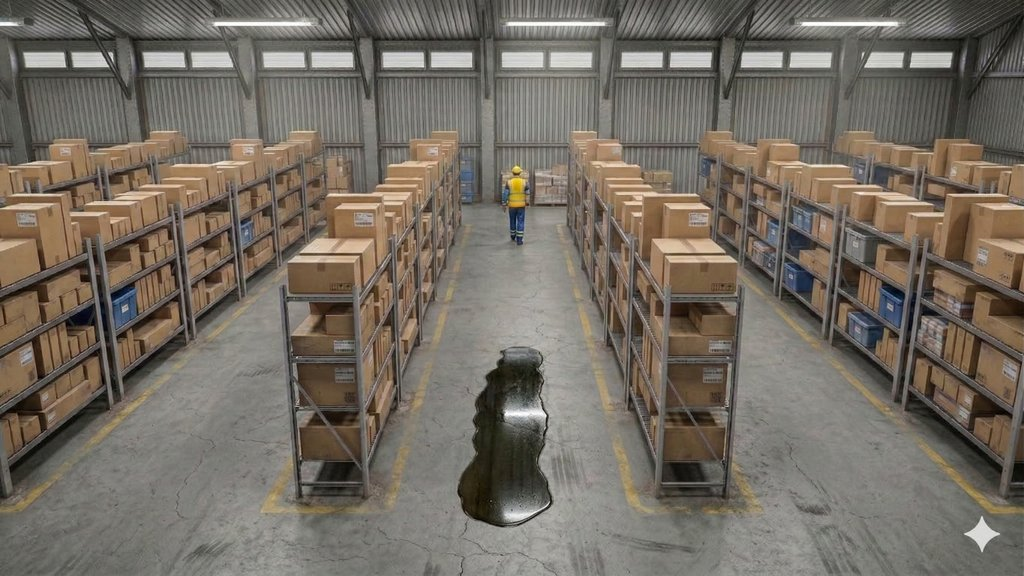
\includegraphics[width=\textwidth]{example_spill.jpg}
        \caption{Spill: dark oil pool with mirror reflections on aisle floor}
    \end{subfigure}
    \hfill
    \begin{subfigure}[b]{0.32\textwidth}
        \centering
        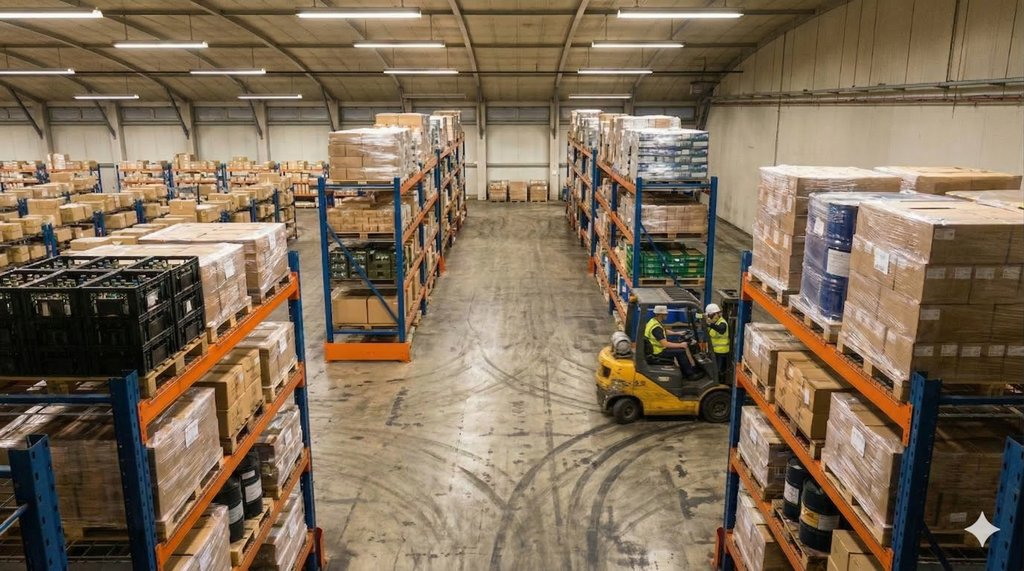
\includegraphics[width=\textwidth]{example_forklift.jpg}
        \caption{Forklift violation: person clinging to front of moving forklift}
    \end{subfigure}
    \hfill
    \begin{subfigure}[b]{0.32\textwidth}
        \centering
        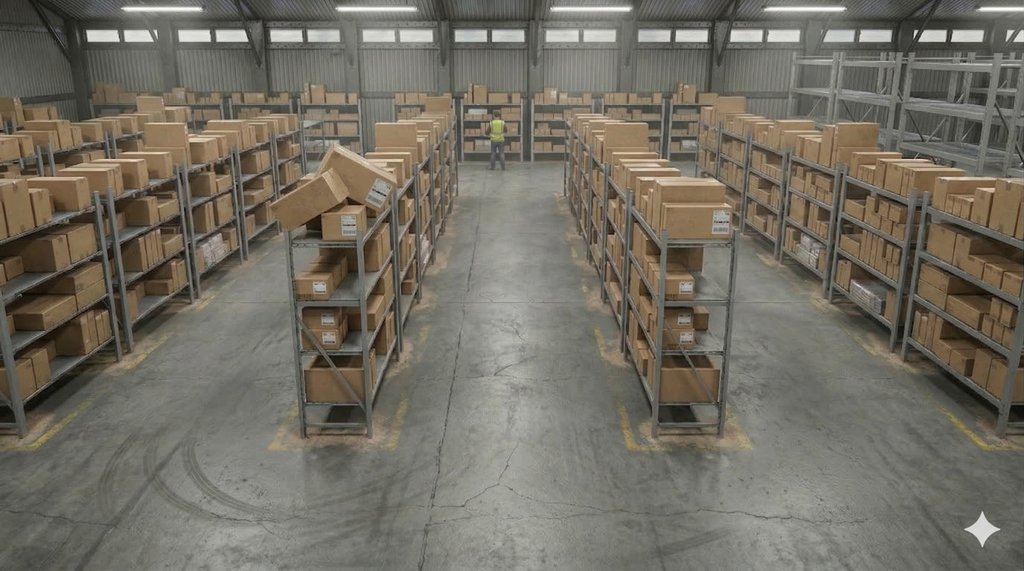
\includegraphics[width=\textwidth]{example_stacking.jpg}
        \caption{Improper stacking: boxes leaning and tilted on upper shelves}
    \end{subfigure}

    \vspace{0.5em}

    \begin{subfigure}[b]{0.32\textwidth}
        \centering
        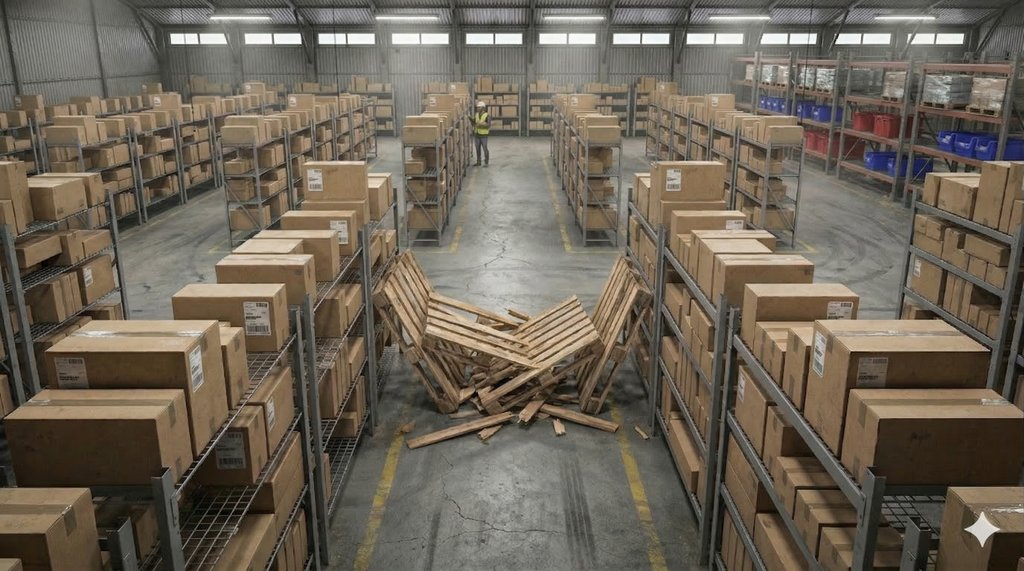
\includegraphics[width=\textwidth]{example_obstacle.jpg}
        \caption{Obstacle: broken pallets blocking the aisle}
    \end{subfigure}
    \hfill
    \begin{subfigure}[b]{0.32\textwidth}
        \centering
        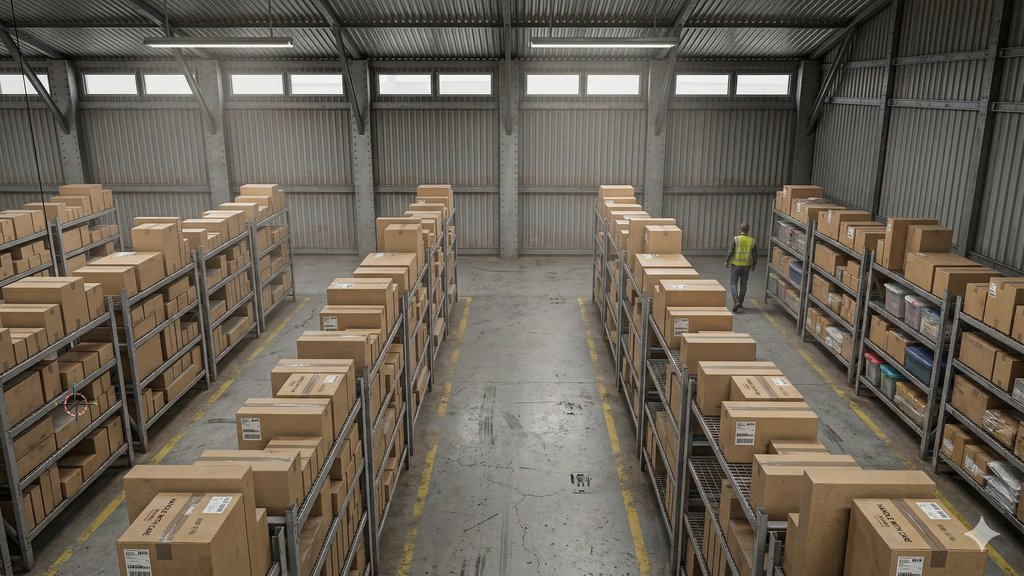
\includegraphics[width=\textwidth]{example_safe.jpg}
        \caption{Safe: clean aisle, orderly shelving, no hazards}
    \end{subfigure}
    \hfill
    \begin{subfigure}[b]{0.32\textwidth}
        \centering
        
\includegraphics[width=\textwidth]{base_render.png}
        \caption{Original Blender render (pre-Gemini)}
    \end{subfigure}
    \caption{Representative examples from each hazard category in the dataset. All images are drone-perspective views generated through the Blender rendering, Gemini photorealistic enhancement, and Gemini hazard injection pipeline. Image (f) shows the raw 3D render before photorealistic conversion.}
    \label{fig:hazards}
\end{figure}

\subsection{Dataset Organization and Labeling}

All 913 images were organized into a structured JSONL metadata file containing category, description, subtype, severity, location, and quality fields. The first author wrote descriptions for each image based on visual observation, and Claude was used to organize these descriptions into the structured metadata format. The first author then personally reviewed all 996 images (before deletion of 83) using a custom HTML review tool with voice-to-text input, correcting 89 categories, adding 124 multi-label tags for dual-hazard images, and writing 242 detailed human observation notes. An additional 8 ground truth corrections were applied during final model verification (Section~\ref{sec:verification}).

% ============================================================
\section{Zero-Shot VLM Benchmark}
\label{sec:benchmark}
% ============================================================

\subsection{Experimental Setup}

We benchmarked nine open-source VLMs on a stratified test set of 150 images (30 per category) on a Mac Mini M4 with 16~GB unified RAM via Ollama. Images were pre-resized to 1024px JPEG. Five prompt strategies were tested (direct classification, OSHA inspector role, chain-of-thought binary questions, describe-then-classify, and JSON structured output). For the top four Qwen 3.5 models, we also tested \textit{think mode} (internal chain-of-thought) versus \textit{nothink mode}. This produced 54 total benchmark runs.

\subsection{Zero-Shot Results}

\begin{table}[H]
\centering
\begin{tabular}{llrrr}
\toprule
\textbf{Model} & \textbf{Best Prompt} & \textbf{Verified Acc.} & \textbf{Time/img} & \textbf{Size} \\
\midrule
Qwen3.5-4B & direct (nothink) & 83.3\% (125/150) & 5.6s & 4.7~GB \\
Qwen3.5-9B & direct (nothink) & 78.0\% (117/150) & 9.0s & 9.7~GB \\
Qwen3.5-2B & direct (nothink) & 65.3\% & 3.1s & 3.78~GB \\
Qwen3.5-0.8B & json\_structured & 64.7\% & 2.1s & -- \\
Gemma3-4B & json\_structured & 63.3\% & 5.3s & 4.3~GB \\
Qwen3-VL-8B & json\_structured & 59.3\% & 18.7s & -- \\
LLaVA-Phi3-4B & direct & 46.0\% & 3.0s & -- \\
Qwen3-VL-2B & direct & 40.7\% & 6.9s & -- \\
Moondream-1B & chain\_of\_thought & 36.7\% & 1.3s & -- \\
\bottomrule
\end{tabular}
\caption{Per-model best accuracy from 54 benchmark runs. Qwen3.5-4B and 9B accuracies were manually verified against updated ground truth. The 4B model outperforms the 9B.}
\label{tab:benchmark}
\end{table}

\subsection{Key Zero-Shot Findings}

\textbf{Finding 1: Smaller can beat larger.} Qwen3.5-4B (83.3\%) outperforms Qwen3.5-9B (78.0\%). The 9B over-classifies, hallucinating hazards from normal floor texture (22 of 33 errors predicted ``obstacle'' from tire marks and concrete stains). The 4B is more conservative. This is significant: more parameters do not always improve performance on domain-specific tasks.

\textbf{Finding 2: Direct prompting wins.} The minimal ``classify into one category'' prompt outperforms elaborate strategies (OSHA role, chain-of-thought, describe-then-classify) across all model sizes. Additional reasoning steps give models room to overthink and second-guess correct initial impressions.

\textbf{Finding 3: Architecture matters more than size.} Qwen 3.5 at every size beats every other architecture at larger sizes. Qwen3.5-0.8B (59.3\%) beats LLaVA-Phi3-4B (46.0\%), a model five times larger.

\textbf{Finding 4: Think mode has a size threshold.} Below 4B, think mode hurts (circular reasoning loops, 11 to 44\% timeout rates). Above 4B, think mode helps (+6 to 15 pp on completed images).

\textbf{Finding 5: Models see but cannot judge.} The 0.8B model's thinking traces reveal it correctly observes ``two workers, one standing near the forks'' but concludes ``looks like normal operation.'' Perception is intact; domain-specific judgment is absent. This is precisely what fine-tuning teaches.

% ============================================================
\section{Fine-Tuning}
% ============================================================

\subsection{Training Data: Multi-Style Conversations}

We generated 2,521 training conversations for 727 training images (80/20 stratified split). The first author personally wrote descriptions for each image based on direct visual observation. These descriptions were then formatted into multi-style training conversations with Claude assisting in organizing the information into the required conversation structures. Three styles were generated per image:

\begin{itemize}
    \item \textbf{Multi-turn Q\&A:} Progressive dialogue (``Is this safe?'' / ``What hazard?'' / ``How severe?'') with negative examples (``Is there a spill?'' / ``No, the floor is dry.'')
    \item \textbf{Direct classification:} Single-turn ``category: X, description: ...''
    \item \textbf{Reasoning chain:} Step-by-step analysis of floor, shelves, forklift, personnel, then conclusion
\end{itemize}

The multi-style approach proved critical. Switching from direct-only to all styles improved accuracy from 78\% to 86\% (+8 pp) in hyperparameter search. The reasoning conversations explicitly teach \textit{why} something is a violation (e.g., ``worker standing near active forks equals OSHA violation''), not just the label.

\subsection{Hyperparameter Search}

Five experiments on a 200-image subset identified the optimal configuration:

\begin{table}[H]
\centering
\begin{tabular}{llrrl}
\toprule
\textbf{Exp} & \textbf{Change} & \textbf{Acc.} & \textbf{Val Loss} & \textbf{Notes} \\
\midrule
1 & lr=1e-4, direct only, 3 epochs & 72\% & 1.07 & Baseline \\
2 & lr=2e-4, direct only & 78\% & 1.26 & +6\% from learning rate \\
3 & lr=2e-4, rank=32 & 76\% & 1.06 & Higher rank overfits \\
\textbf{4} & \textbf{lr=2e-4, all styles, 3 epochs} & \textbf{86\%} & \textbf{1.05} & \textbf{+8\% from multi-style data} \\
5 & lr=2e-4, all styles, 5 epochs & 82\% & 1.20 & Overfits at epoch 4+ \\
\bottomrule
\end{tabular}
\caption{Hyperparameter search on 200-image subset (50 validation images). Multi-style training data was the single most impactful change.}
\end{table}

Final configuration: learning rate 2e-4, LoRA rank 16, alpha 32, dropout 0.05, all linear layers (including vision encoder), 3 epochs, all conversation styles.

\subsection{Full Training}

Training was performed on Kaggle using a free NVIDIA T4 GPU (16~GB VRAM):

\begin{itemize}
    \item \textbf{Framework:} Unsloth + HuggingFace TRL SFTTrainer
    \item \textbf{Base model:} Qwen3.5-2B (2.3 billion parameters)
    \item \textbf{Precision:} float32
    \item \textbf{LoRA adapter size:} 88~MB (1.1\% of base model parameters)
    \item \textbf{Training data:} 2,521 conversations (727 images, approximately 3.5 styles each)
    \item \textbf{Label masking:} Only assistant response tokens trained (89\% prompt masked, 11\% response trained)
    \item \textbf{Training time:} 3.5 hours
    \item \textbf{Final loss:} 0.714 (from 1.733 at step 25)
    \item \textbf{Cost:} \$0 (Kaggle free tier)
\end{itemize}

\subsection{Deployment and Quantization}

The LoRA adapter was merged with the base model and converted to GGUF format for deployment via Ollama on a Mac Mini M4 with 16~GB RAM.

\begin{table}[H]
\centering
\begin{tabular}{lrl}
\toprule
\textbf{Component} & \textbf{Size} & \textbf{Format} \\
\midrule
Original merged model & 8.3~GB & float32 \\
Quantized language model & 1.2~GB & Q4\_K\_M (4-bit k-quant medium) \\
Vision encoder & 637~MB & F16 (not quantized, preserves visual detail) \\
\midrule
\textbf{Total deployed model} & \textbf{1.8~GB} & \textbf{78\% size reduction} \\
\bottomrule
\end{tabular}
\caption{Model sizes. The vision encoder is kept at F16 because quantizing it degrades image understanding. The language model handles quantization well for classification output.}
\end{table}

% ============================================================
\section{Evaluation and Verification}
\label{sec:verification}
% ============================================================

\subsection{Manual Verification Protocol}

All accuracy figures in this work were verified by manually reading every model response for every test image. This was necessary because automated evaluation parsers contained significant bugs. The most severe: the base model's Kaggle evaluation script matched ground truth keywords anywhere in the response text, including negations (``I see no spill'' matched ``spill''), inflating reported accuracy from 67.2\% to 84.9\%.

For each of 186 test images, across six model configurations (base 2B think, base 4B nothink, base 9B nothink, fine-tuned Q4 nothink, fine-tuned Q4 think, fine-tuned F32 nothink), we:

\begin{enumerate}
    \item Read the ground truth category, description, human notes, and accept\_also fields
    \item Read the model's complete response (including think-mode reasoning)
    \item Determined the model's actual final classification by reading, not keyword matching
    \item Verified the model's observations against what is visible in the image
    \item For disputed cases, visually inspected the actual image
\end{enumerate}

This process identified 8 ground truth labels that were incorrect (the model was right, the GT was wrong), which were corrected in the dataset.

\subsection{Results}

\begin{table}[H]
\centering
\begin{tabular}{lrrrl}
\toprule
\textbf{Model Configuration} & \textbf{Correct} & \textbf{Accuracy} & \textbf{Time/img} & \textbf{Size} \\
\midrule
\textbf{Fine-tuned F32 (nothink)} & \textbf{175/186} & \textbf{94.1\%} & 150.6s & 8.3~GB \\
\textbf{Fine-tuned Q4 (think)} & \textbf{172/186} & \textbf{92.5\%} & 4.2s & 1.8~GB \\
\textbf{Fine-tuned Q4 (nothink)} & \textbf{171/186} & \textbf{91.9\%} & 2.9s & 1.8~GB \\
\midrule
Zero-shot Qwen3.5-4B (nothink) & 125/150 & 83.3\% & 5.6s & 4.7~GB \\
Zero-shot Qwen3.5-9B (nothink) & 117/150 & 78.0\% & 9.0s & 9.7~GB \\
Zero-shot Qwen3.5-2B (think) & 125/186 & 67.2\% & -- & 3.78~GB \\
Zero-shot Qwen3.5-2B (nothink) & -- & 65.3\% & 3.1s & 3.78~GB \\
\bottomrule
\end{tabular}
\caption{All figures manually verified. The 1.8~GB quantized model outperforms zero-shot models up to 5.4 times its size while running faster. F32 = full precision (float32). Q4 = Q4\_K\_M quantization.}
\label{tab:results}
\end{table}

\subsection{Quantization Analysis}

Quantizing from 8.3~GB to 1.8~GB costs only 2.2 percentage points (94.1\% to 91.9\%) while providing 78\% size reduction and 52x speed improvement. The quantized model with think mode (92.5\%) nearly matches the full-precision nothink model (94.1\%) at 36x faster inference. This demonstrates that aggressive quantization is practical for deployment-critical applications.

\subsection{Think Mode Analysis}

Think mode on the quantized model improves accuracy by 0.6 pp (91.9\% to 92.5\%) with only 1.3 additional seconds per image. The fine-tuned model produces zero timeouts or infinite reasoning loops, unlike the base model which timed out on 11 to 44\% of images. Think mode specifically recovers 7 images involving subtle forklift violations (tipping angles, unsecured loads, distant pedestrians) where step-by-step reasoning identifies details that quick classification misses.

% ============================================================
\section{Qualitative Analysis}
% ============================================================

\subsection{Base Model vs. Fine-Tuned: Pedestrian Proximity}

The most striking qualitative difference is in forklift pedestrian proximity detection. The base model consistently sees workers near forklifts but judges the situation as safe. The fine-tuned model has learned that proximity to active forklifts constitutes a violation. Below we show three test images with the full responses from both models side by side.

\vspace{1em}
\noindent\textbf{Comparison 1:} Person clinging to front of moving forklift (Ground truth: forklift\_violation)

\begin{figure}[H]
\centering
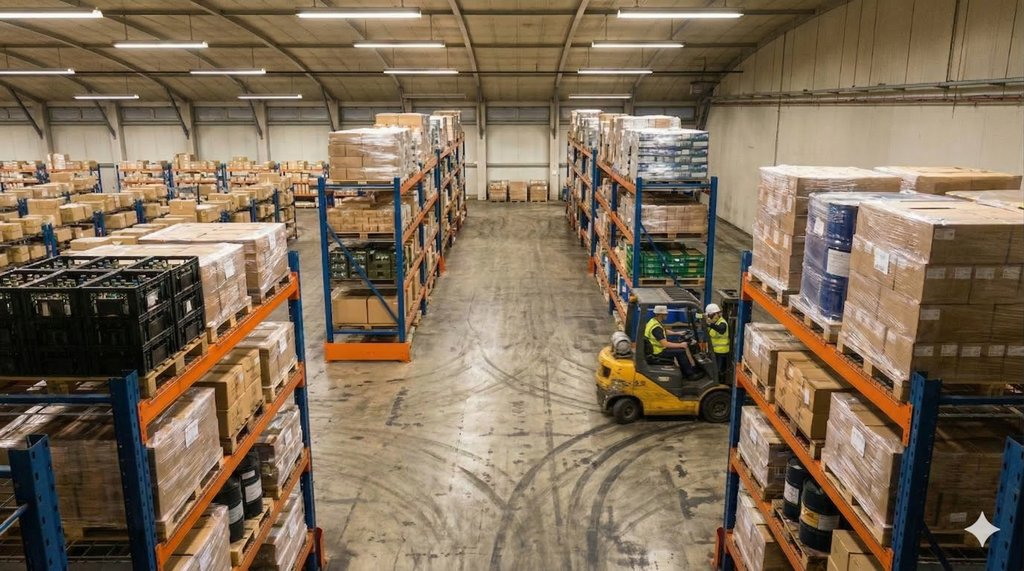
\includegraphics[width=0.45\textwidth]{compare_forklift_0004.jpg}
\end{figure}
\vspace{-0.5em}

\noindent
\begin{tabular}{@{}p{0.48\textwidth}|p{0.48\textwidth}@{}}
\textbf{Base Qwen3.5-2B} \textcolor{red}{WRONG} & \textbf{Fine-tuned (Ours)} \textcolor{green!60!black}{CORRECT} \\
\hline
``There are no identifiable safety hazards present. The forklift is operating within safe limits, personnel are properly equipped.'' \newline \textbf{Classification: safe} &
``Two workers visible on or near the forklift. One appears to be operating while another is riding on or clinging to the side. This unauthorized rider situation violates safe forklift operation protocols.'' \newline \textbf{Classification: forklift\_violation} \\
\end{tabular}

\vspace{1.5em}
\noindent\textbf{Comparison 2:} Worker standing on elevated forks at height (Ground truth: forklift\_violation)

\begin{figure}[H]
\centering
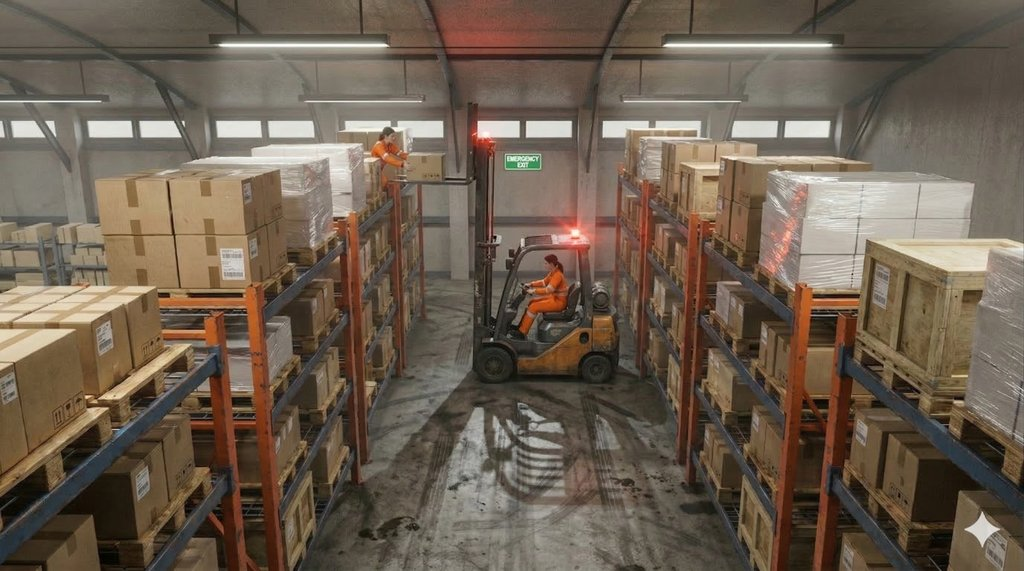
\includegraphics[width=0.45\textwidth]{compare_forklift_0145.jpg}
\end{figure}
\vspace{-0.5em}

\noindent
\begin{tabular}{@{}p{0.48\textwidth}|p{0.48\textwidth}@{}}
\textbf{Base Qwen3.5-2B} \textcolor{red}{WRONG} & \textbf{Fine-tuned (Ours)} \textcolor{green!60!black}{CORRECT} \\
\hline
``The environment is functional and does not exhibit any critical safety issues. Therefore: safe.'' \newline \textbf{Classification: safe} &
``A worker in an orange jumpsuit is standing on the elevated forks of the forklift itself, reaching toward upper shelf levels. This is an unauthorized riding violation -- forklifts are designed for seat operation only, not as personal elevators.'' \newline \textbf{Classification: forklift\_violation} \\
\end{tabular}

\vspace{1.5em}
\noindent\textbf{Comparison 3:} Pedestrian walking alongside moving forklift (Ground truth: forklift\_violation)

\begin{figure}[H]
\centering
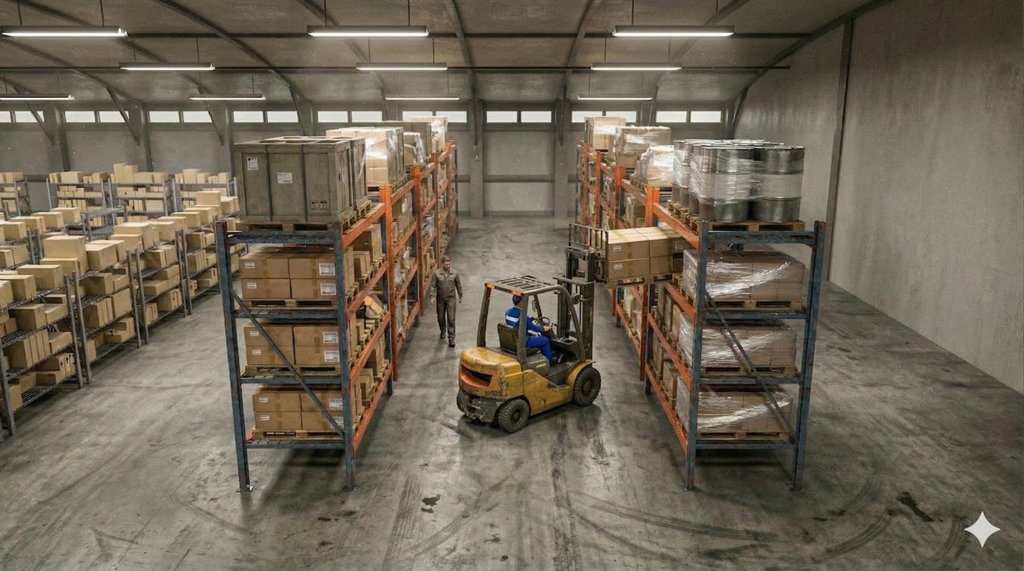
\includegraphics[width=0.45\textwidth]{compare_forklift_0051.jpg}
\end{figure}
\vspace{-0.5em}

\noindent
\begin{tabular}{@{}p{0.48\textwidth}|p{0.48\textwidth}@{}}
\textbf{Base Qwen3.5-2B} \textcolor{red}{WRONG} & \textbf{Fine-tuned (Ours)} \textcolor{green!60!black}{CORRECT} \\
\hline
``There are no identifiable safety hazards present. The forklift is operating correctly, personnel are behaving appropriately.'' \newline \textbf{Classification: safe} &
``A pedestrian worker in a grey uniform walks in close proximity on the left side. The worker is within the forklift's operating zone, violating safe separation requirements between powered industrial vehicles and foot traffic.'' \newline \textbf{Classification: forklift\_violation} \\
\end{tabular}

\label{tab:qualitative}

\vspace{1em}
\noindent In all three cases, the base model perceives the workers but lacks the domain knowledge to judge proximity as dangerous. The fine-tuned model learned OSHA safety standards from the multi-style training conversations, specifically that pedestrians within the forklift's operating zone constitute a violation regardless of whether the forklift ``appears to be operating correctly.''

\subsection{Description Quality}

The fine-tuned 2.3B model produces descriptions that demonstrate genuine domain understanding:

\begin{itemize}
    \item \textbf{Reads text in images:} Identifies ``FRAGILE,'' ``THIS SIDE UP,'' ``CAUTION FORKLIFT TRAFFIC,'' ``8 km/h'' speed signs
    \item \textbf{Identifies specific materials:} ``amber-brown oil,'' ``blue plastic container,'' ``splintered wooden planks,'' ``grey cylindrical container''
    \item \textbf{Accurate spatial reasoning:} ``lower-left foreground near base of left shelving,'' ``at the corner of the aisle row''
    \item \textbf{Explains safety reasoning:} ``unauthorized riding violation -- forklifts are designed for seat operation only''
    \item \textbf{Recognizes dual hazards:} ``The combination of the liquid spill and the displaced box creates both a slip hazard and an obstacle''
\end{itemize}

Representative response (forklift\_0088, person clinging to a moving forklift):

\begin{quote}
\textit{``A yellow forklift is operating in a warehouse aisle between tall orange pallet racks. A worker is hanging onto the rear frame of the forklift, riding on the back of the vehicle as it moves through the aisle. This is an extremely dangerous unauthorized riding situation with no seatbelt or safety restraint. The operator is seated at the controls while the second person clings to the rear of the moving vehicle.''}
\end{quote}

This is not template filling or keyword matching. The model observes specific visual details, identifies the hazard, explains why it is dangerous, and notes contributing factors.

\subsection{Error Analysis}

The 14 errors from the quantized think mode model (7.5\% error rate) fall into categories that represent genuine detection challenges:

\begin{enumerate}
    \item \textbf{Safe over-detection (5):} Minor shelf unevenness or floor marks interpreted as hazards. One error involves misjudging pedestrian distance from a compressed drone perspective.
    \item \textbf{Wrong hazard category (3):} Model identifies something wrong but picks the wrong category (e.g., sees floor debris but classifies as forklift violation instead of obstacle).
    \item \textbf{Missed subtle visual cues (3):} Distant spills barely visible at drone altitude, torn shrink wrap in dim lighting, stacking irregularities obscured by overhead angle.
    \item \textbf{Ambiguous forklift situations (2):} Forks raised during what could be normal shelving operations; unsecured barrel straps invisible at image resolution.
    \item \textbf{Output format edge case (1):} Correct reasoning but unparseable output format.
\end{enumerate}

A human OSHA inspector standing in the aisle would likely catch all of these. From an overhead drone image at 1024px resolution, they represent the practical limit of visual detection.

% ============================================================
\section{Discussion}
% ============================================================

\subsection{The Synthetic Specialization Pipeline}

The central contribution is the pipeline, not the model checkpoint. For warehouse safety specifically:

\begin{enumerate}
    \item Blender 3D scene (or facility camera images) provides the base environment
    \item Gemini image editing injects hazards with randomized prompts
    \item Claude generates structured metadata and multi-style training conversations
    \item Unsloth + LoRA fine-tunes a 2B VLM on Kaggle (free T4, 3.5 hours)
    \item Q4\_K\_M quantization compresses to 1.8~GB for edge deployment
\end{enumerate}

A different facility would repeat steps 1 through 5 with its own images. The model does not need to generalize across facilities because the pipeline makes specialization cheap.

\subsection{Why Small Fine-Tuned Beats Large Generic}

Our results show a 25.3 percentage point improvement from fine-tuning (67.2\% to 92.5\%), with the 1.8~GB fine-tuned model outperforming zero-shot models up to 9.7~GB. This is explained by the nature of the task:

\begin{itemize}
    \item \textbf{Domain knowledge gap:} General-purpose VLMs know ``forklifts exist'' but not ``pedestrians within 3 meters of an active forklift is an OSHA violation.'' Fine-tuning injects this domain knowledge.
    \item \textbf{Environment specificity:} The fine-tuned model learns this specific warehouse's floor texture, shelving style, lighting conditions, and camera angle. It stops hallucinating spills from normal concrete stains.
    \item \textbf{Output calibration:} Multi-style training teaches the model a structured output format, eliminating the verbose, ambiguous responses that cause parsing errors in zero-shot evaluation.
\end{itemize}

\subsection{VLM vs. CNN for Contextual Tasks}

\begin{table}[H]
\centering
\begin{tabular}{lll}
\toprule
& \textbf{CNN (e.g., YOLOv8)} & \textbf{VLM (our approach)} \\
\midrule
Training data needed & 2,500--10,000 with bounding boxes & 727 with text descriptions \\
Annotation cost & Manual bbox labeling & Automatic from injection process \\
Real hazard photos needed & Yes, ideally & No (synthetic works) \\
New facility & Retrain from scratch & Re-run pipeline with new images \\
Output & Bounding box + class label & Natural language explanation \\
Novel hazard types & Cannot detect (only trained classes) & Can describe anything unusual \\
Inference speed & 30+ FPS & 2.9--4.2 seconds/image \\
\bottomrule
\end{tabular}
\caption{For periodic safety checks (every 5--10 seconds), VLM latency is acceptable, and the explanatory output is more useful to safety officers than a bounding box.}
\end{table}

\subsection{Limitations}

\begin{enumerate}
    \item \textbf{Single environment:} All images come from one Blender warehouse scene. The model has not been validated on real photographs or different layouts.
    \item \textbf{Drone perspective only:} Training used overhead images at approximately 55 degrees. Wall-mounted cameras would require new training data.
    \item \textbf{Synthetic data gap:} Despite photorealism, subtle differences from real camera feeds may exist.
    \item \textbf{Five categories only:} Missing PPE, fire risks, and electrical hazards are not covered.
    \item \textbf{No cross-environment generalization:} By design, the model specializes to one facility. This is a feature (high accuracy) and a limitation (requires pipeline re-run for new sites).
\end{enumerate}

% ============================================================
\section{Computational Resources}
% ============================================================

\begin{table}[H]
\centering
\begin{tabular}{lll}
\toprule
\textbf{Task} & \textbf{Platform} & \textbf{Cost} \\
\midrule
3D scene construction and rendering & MacBook Pro M2 16~GB (Blender 5.0.1) & \$0 \\
Image generation (999 images) & Google Gemini Pro subscription & \$25/month \\
Dataset labeling and metadata & Claude (annotation and organization) & Included \\
Zero-shot benchmarking (54 runs) & Mac Mini M4 16~GB (Ollama) & \$0 \\
Training data generation (2,521 conversations) & First author wrote descriptions; Claude assisted with formatting & Included \\
Hyperparameter search (5 experiments) & Kaggle free T4 GPU & \$0 \\
Full model training (3.5 hours) & Kaggle free T4 GPU & \$0 \\
Model deployment and evaluation & Mac Mini M4 16~GB (Ollama) & \$0 \\
\midrule
\textbf{Total compute cost} & & \textbf{approximately \$25} \\
\bottomrule
\end{tabular}
\caption{The entire pipeline runs on consumer hardware and free cloud services. No proprietary datasets, no paid GPU clusters, no enterprise APIs required for training or deployment.}
\end{table}

% ============================================================
\section{Future Work}
% ============================================================

\subsection{Planned Experiments (SHARCNET H100 GPUs)}

Access to NVIDIA H100 GPUs through Alliance Canada (SHARCNET) enables several planned experiments:

\begin{enumerate}
    \item \textbf{Data efficiency curve:} Training on 100, 200, 400, and 727 images for both Qwen3.5-2B and Qwen3.5-4B models with 3 random seeds each (24 runs total). This determines the minimum viable dataset size and produces the most practically useful result for other researchers adopting this approach.
    \item \textbf{Training style ablation:} Systematic comparison of direct-only, multi-turn-only, reasoning-only, and mixed training data (12 runs with 3 seeds). No prior work has studied how conversation format diversity affects domain-specific VLM performance.
    \item \textbf{LoRA rank sweep:} Ranks 4, 8, 16, 32, 64 to identify diminishing returns.
    \item \textbf{2B vs. 4B model comparison:} Full training of both model sizes with identical configuration to measure parameter efficiency.
\end{enumerate}

\subsection{Broader Pipeline Validation}

\begin{enumerate}
    \item \textbf{Real-world testing:} Evaluating the warehouse model on actual facility camera footage to measure the synthetic-to-real transfer gap.
    \item \textbf{Cross-domain application:} Applying the synthetic specialization pipeline to a different domain (e.g., construction safety, retail loss prevention, agricultural crop disease) to validate that the approach generalizes beyond warehouses.
    \item \textbf{Automated pipeline engine:} Building a tool where users provide facility images, select hazard categories, and the system automatically generates training data, fine-tunes a model, and produces a deployable checkpoint. This is the ultimate realization of the synthetic specialization vision.
\end{enumerate}

% ============================================================
\section{Conclusion}
% ============================================================

We have demonstrated \textit{synthetic specialization}: a pipeline where AI-generated synthetic data is used to fine-tune and compress a small foundation model into a domain-specific expert. Applied to warehouse safety hazard detection:

\begin{itemize}
    \item A 1.8~GB quantized model achieves 92.5\% accuracy, outperforming zero-shot models up to 5.4x its size
    \item The full-precision variant reaches 94.1\%, a 26.9 percentage point improvement over the base architecture
    \item The fine-tuned model specifically learns contextual safety reasoning (e.g., pedestrian proximity to forklifts) that no zero-shot model captures
    \item The entire pipeline costs approximately \$25 and runs on consumer hardware
    \item Think mode adds 2.7\% accuracy with no timeouts, unlike base models which timeout on 11--44\% of images
\end{itemize}

The key finding extends beyond warehouse safety: \textit{small fine-tuned models consistently beat large generic models when training data matches the deployment context}. This suggests a practical paradigm for any domain where real training data is scarce, dangerous, or expensive to collect, but the target environment is known and can be simulated. Rather than scaling model size to cover every possible scenario, we can scale data specificity to cover the one scenario that matters.

The vision for this work is an engine where any organization can point at their facility, generate synthetic training data tailored to their environment, and produce a specialized AI model that works for them, without machine learning expertise, without real hazard data, and without expensive infrastructure. This case study proves the core pipeline works.

% ============================================================
\begin{thebibliography}{99}

\bibitem{synspill2025}
A.~Baranwal, A.~Mueez, J.~Voelker, G.~Bhatia, and S.~Vyas, ``SynSpill: Improved Industrial Spill Detection With Synthetic Data,'' in \textit{Proc. ICCV Workshop (VISION'25)}, 2025.

\bibitem{bladeSynth2025}
BladeSynth Authors, ``BladeSynth: A High-Quality Rendering-Based Synthetic Dataset for Aero Engine Blade Defect Inspection,'' \textit{Scientific Data (Nature)}, 2025.

\bibitem{syngenVision2025}
SynGen-Vision Authors, ``SynGen-Vision: Synthetic Data Generation for Training Industrial Vision Models,'' \textit{arXiv:2509.04894}, 2025.

\bibitem{tfidg2025}
Y.~Xu et al., ``Training-Free Industrial Defect Generation with Diffusion Models,'' in \textit{Proc. ICCV}, 2025.

\bibitem{isafetybench2025}
R.~Abdullah, Y.~S.~Rawat, and S.~Vyas, ``iSafetyBench: A Video-Language Benchmark for Safety in Industrial Environments,'' in \textit{Proc. ICCV Workshop (VISION'25)}, 2025.

\bibitem{constructionVLM2025}
ConstructionSite 10k Authors, ``Are Large Pre-Trained Vision Language Models Effective Construction Safety Inspectors?'' \textit{arXiv:2508.11011}, 2025.

\bibitem{monitorVLM2025}
H.~Wu et al., ``MonitorVLM: A Vision-Language Framework for Safety Violation Detection in Mining Operations,'' \textit{arXiv:2510.03666}, 2025.

\bibitem{excavatorVLM2025}
Excavator VLM Authors, ``Resource-Efficient Fine-Tuning of Large Vision-Language Models for Multimodal Perception in Autonomous Excavators,'' \textit{Frontiers in Artificial Intelligence}, 2025.

\bibitem{compactVLMbenchmark2025}
Compact VLM Benchmark Authors, ``Benchmarking Compact VLMs for Clip-Level Surveillance Anomaly Detection Under Weak Supervision,'' \textit{Journal of Imaging}, vol.~11, no.~11, 2025.

\bibitem{hu2022lora}
E.~J.~Hu et al., ``LoRA: Low-Rank Adaptation of Large Language Models,'' in \textit{Proc. ICLR}, 2022.

\bibitem{dettmers2023qlora}
T.~Dettmers, A.~Pagnoni, A.~Holtzman, and L.~Zettlemoyer, ``QLoRA: Efficient Finetuning of Quantized Language Models,'' in \textit{Proc. NeurIPS}, 2023.


\end{thebibliography}

\end{document}
